\chapter{Charge pump regulation}
\section{Theory and related work} \label{sec:literature_chargepump}
A charge pump is an electronic circuit that converts a supply voltage to a DC output voltage that is several times higher. Unlike the other traditional DC-DC converters, which employ inductors, charge pumps are only made of capacitors and switches (implemented by diodes or MOSFETs) \cite{chargepump-article}. The arrangement of these switches, allows for the charge pump to be used as a voltage doubler (or multiplier with extra stages) or as a voltage inverter \cite{chargepump-main}.
\section{Design} \label{sec:design_chargepump}
\textbf{\textit{Design rationale}}
As standard diodes are to be used as the switches in the design, the diode voltage drops have to be accounted for \cite{chargepump-main}. This means that the \SI{5}{\volt} amplitude clock cannot be connected directly into the charge pump scheme if a \SI{-5}{\volt} output is to be achieved. Thus, an amplifier stage is implemented to boost the clock to a sufficiently high amplitude. 

This is achieved using one of the provided BJTs. In order to provide isolation to the amplifier stage, a pair of BJTs are connected between the amplifier and the charge pump. These are set to alternatively switch on and off, thus providing a path for current to flow during charging and discharging of the charge pump's flying capacitor without affecting the operation of the amplifier. To achieve this alternate switching, the amplifier is designed to be inverting and its output connected to the first of the transistors. The second switching transistor is then connected to the input clock to finalise the transistor switching scheme. 

The amplifying transistor is designed to be in saturation or cutoff, to maximise its output \cite{Neamen:Microelectronics}. The switching transistors only had a base resistor, as this helped to increase the efficiency of the charge pump. All the resistors were adjusted in simulation such that the charge pump could supply enough current to its load. Reducing the size of the resistors helped achieve this. 

The arrangement of the capacitors and diodes was obtained from \cite{chargepump-main}. The capacitors should be large enough to store the charge lost to the load each cycle, but not so large that they cannot fully charge up. From Figure \ref{fig:chargepump_circuit}, C4 should be larger than C7 as it has to supply charge to the load, as well as charge up capacitor C7 when it discharges. C7 has to be large enough to avoid a significant ripple appearing at the output. 

To provide some load regulation to the charge pump, a Zener diode is connected to its output \cite{Neamen:Microelectronics}. This clips the output at \SI{-5}{\volt} irregardless of the load connected. Since the charge pump is designed for a maximum load of \SI{25}{\milli\ampere}, there is no risk of exceeding the power rating of the Zener. Finally, a filter is connected to the output of the charge pump. This helps remove the \SI{10}{\kilo Hz} noise induced by the clock, as well as any \SI{150}{\kilo Hz} noise from the switchmode regulator.


\noindent\textbf{textit{Design calculations}}


\noindent\textbf{\textit{Circuit diagram}}
 
\begin{figure}[h] 
 \centering
  	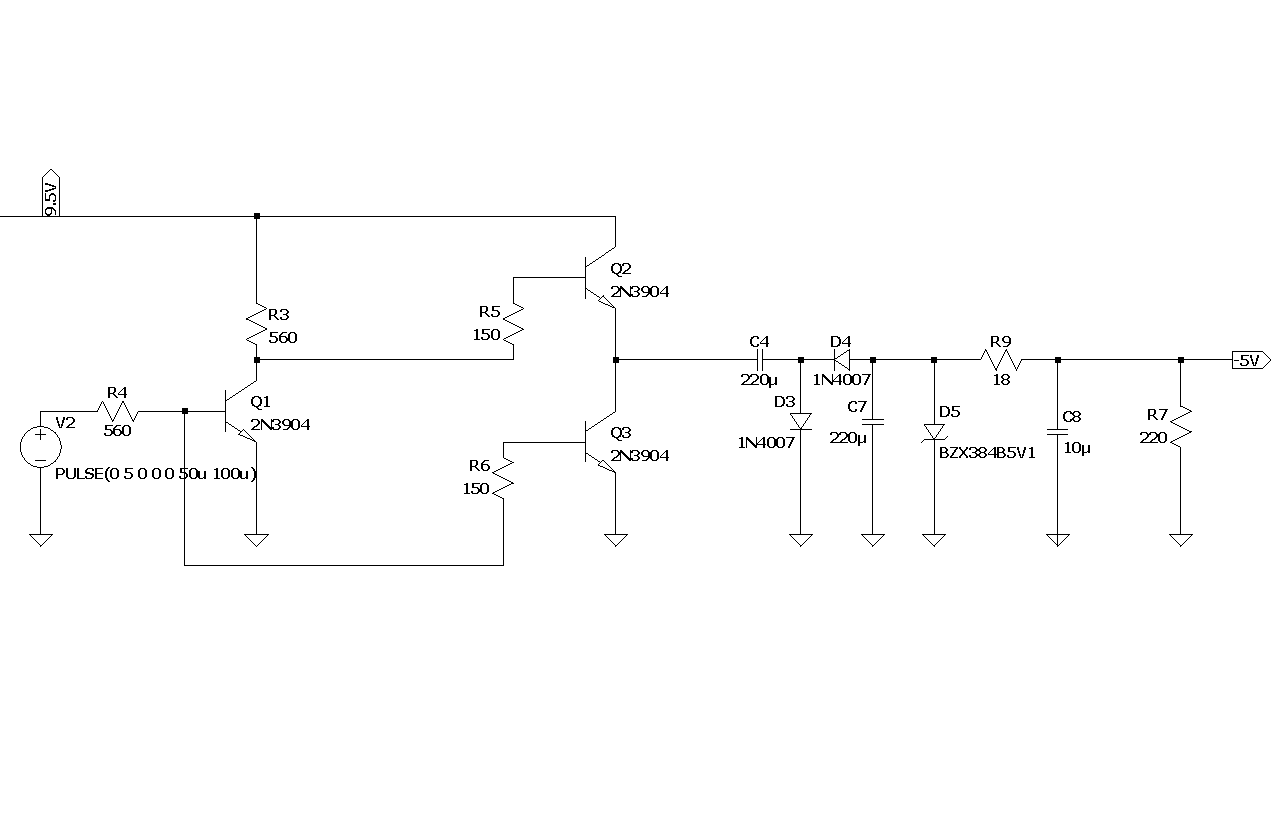
\includegraphics[clip, trim = 0cm 4.2cm 0cm 2.8cm, width=1\linewidth]{./Figures/chargepump_circuit.pdf}
  	\caption{Charge pump circuit.}
  	\label{fig:chargepump_circuit}
 \end{figure}
 
 

\section{Simulation} \label{sec:simulation_chargepump}
\begin{figure} 
 \centering
  	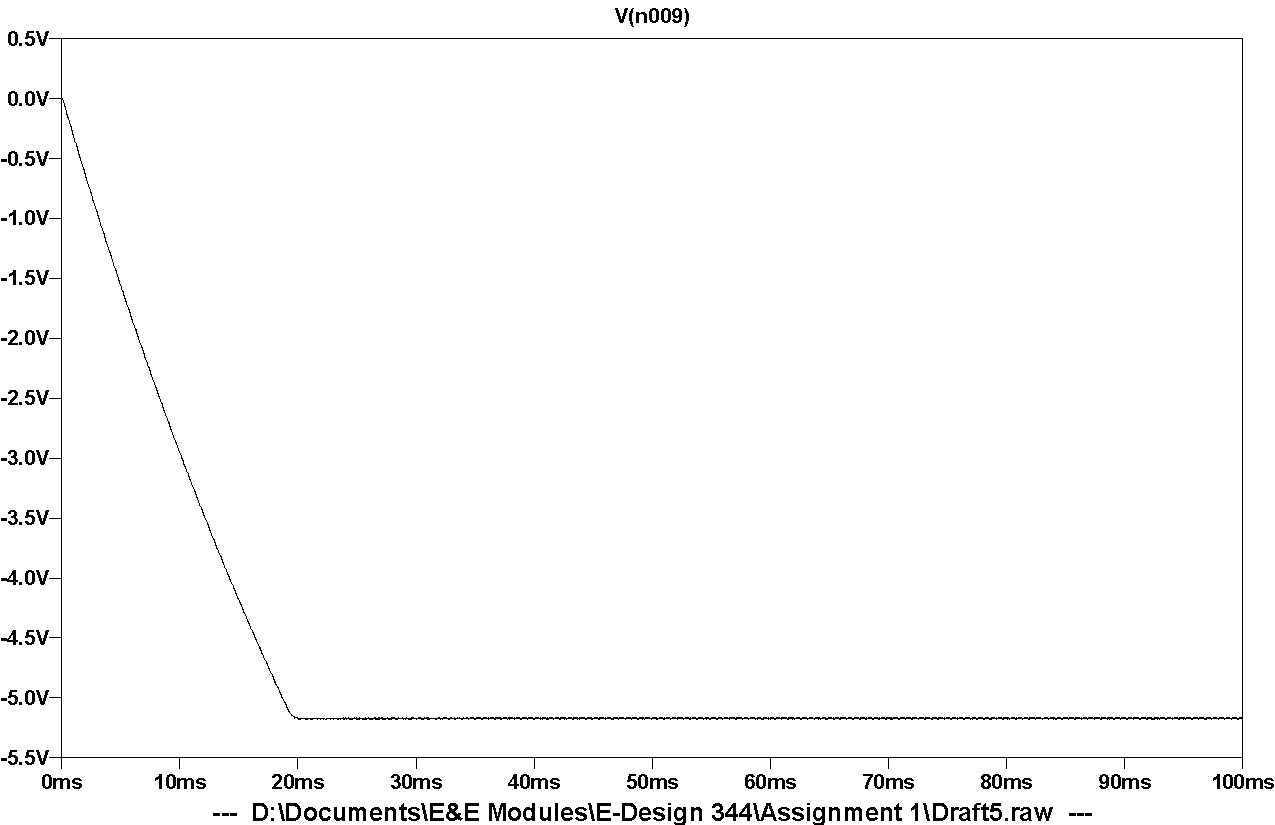
\includegraphics[width=0.6\linewidth]{./Figures/chargepump_simulate.pdf}
  	\caption{Simulated +5V output.}
  	\label{fig:-5v_simulation}
 \end{figure}
 
 
\section{Measurements} \label{sec:measurements_chargepump}
\begin{figure} 
 \centering
 
    \begin{subfigure}[]{0.49\linewidth}
        \centering
        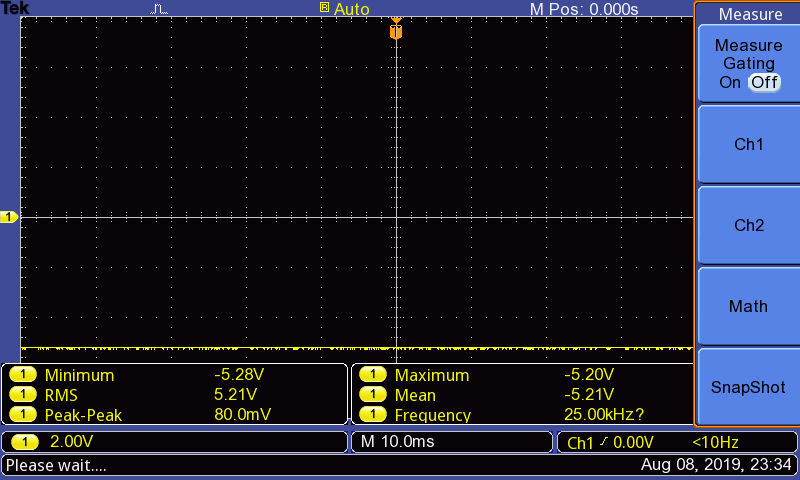
\includegraphics[width=1.\linewidth,clip, trim = 0cm 0cm 2.5cm 0cm]{./Figures/-5v_test}
        \caption{-5V output voltage}
        \label{fig:-5v_output_measurement}
    \end{subfigure}
    \begin{subfigure}[]{0.49\linewidth}
        \centering
        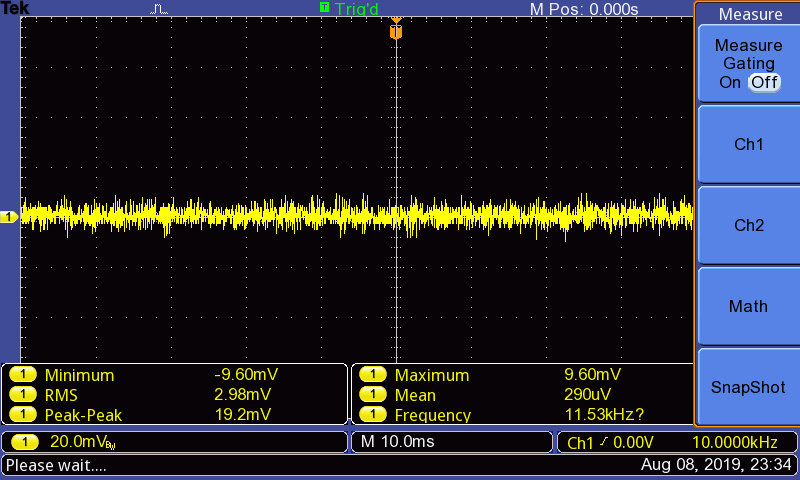
\includegraphics[width=1.\linewidth,clip, trim = 0cm 0cm 2.5cm 0cm]{./Figures/-5v_noise_test}
        \caption{-5V noise levels.}
        \label{fig:-5v_noise_measurement}
    \end{subfigure}
    
\caption{-5V measured output}
\label{fig:-5v_measurement_box}
\end{figure}









